% Created 2021-01-25 Mon 10:29
% Intended LaTeX compiler: pdflatex
\documentclass[11pt]{article}
\usepackage[utf8]{inputenc}
\usepackage[T1]{fontenc}
\usepackage{graphicx}
\usepackage{grffile}
\usepackage{longtable}
\usepackage{wrapfig}
\usepackage{rotating}
\usepackage[normalem]{ulem}
\usepackage{amsmath}
\usepackage{textcomp}
\usepackage{amssymb}
\usepackage{capt-of}
\usepackage{hyperref}
\usepackage{minted}
\hypersetup{colorlinks=true, linkcolor=black, filecolor=red, urlcolor=blue}
\usepackage[turkish]{babel}
\author{Eren Hatırnaz}
\date{28 Temmuz 2019}
\title{Yazılım Gündemi - 3\\\medskip
\large 22-28 Temmuz 2019}
\hypersetup{
 pdfauthor={Eren Hatırnaz},
 pdftitle={Yazılım Gündemi - 3},
 pdfkeywords={},
 pdfsubject={},
 pdfcreator={Emacs 27.1 (Org mode 9.3)},
 pdflang={Turkish}}
\begin{document}

\maketitle
\tableofcontents \clearpage\shorthandoff{=}

\begin{center}
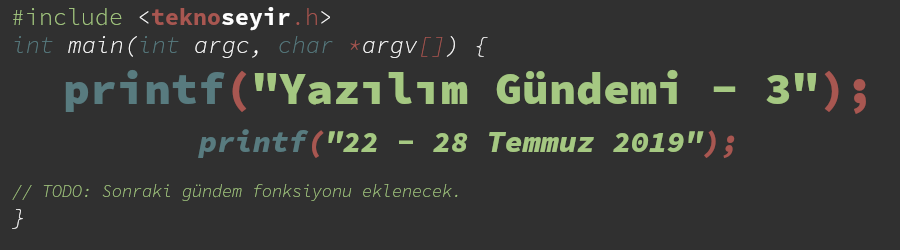
\includegraphics[width=.9\linewidth]{gorseller/yazilim-gundemi-banner.png}
\end{center}

\begin{center}
\href{../02/yazilim-gundemi-02.pdf}{< Önceki Gündem} | \textbf{22-28 Temmuz 2019} | \href{../04/yazilim-gundemi-04.pdf}{Sonraki Gündem >}

\href{https://teknoseyir.com/blog/yazilim-gundemi-3-22-28-temmuz-2019}{TeknoSeyir'de Oku}
\end{center}

\section{GitHub, Amerika yaptırımlarını \href{https://help.github.com/en/articles/github-and-trade-controls}{uygulamaya başladı}}
\label{sec:orgd8c945b}
\begin{figure}[htbp]
\centering
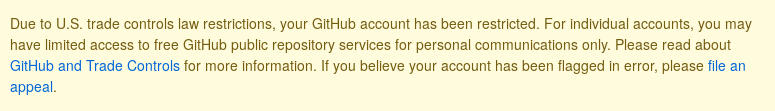
\includegraphics[width=.9\linewidth]{gorseller/github-amerika-yaptirimlari-1.png}
\caption{Kısıtlanan kullanıcıların ekranlarında çıkan uyarı metini}
\end{figure}

GitHub bu kararları yeni mi uygulamaya başladı, yoksa daha önceden de
uygulanıyordu fakat bu kadar sert mi değildi, bilemiyorum fakat bu hafta
birkaç olaya karıştığı için gündem oldu. Bu olaylar şu şekilde:

\begin{itemize}
\item \textbf{Kırımlı bir geliştiricinin \href{https://github.com/tkashkin/GameHub/issues/289}{GitHub hesabının kısıtlanması}}
\item \textbf{Iranlı bir geliştiricinin \href{https://medium.com/hamed/github-blocked-my-account-and-they-think-im-developing-nuclear-weapons-e7e1fe62cb74}{GitHub hesabının kısıtlanması}}
\end{itemize}

Kısıtlamaların tam listesi olmamakla birlikte geliştiricilerin şu an maruz
kaldıkları kısıtlamalar bu şekilde:

\begin{itemize}
\item GitHub Pages üzerinde barındırdıkları web siteleri ulaşılamaz oldu (GitHub
404 sayfası gönderiyor).
\item Yeni özel depo oluşturamıyorlar.
\item Var olan özel depolarına erişemiyorlar. \texttt{git clone} komutu da 403 kodu
dönüyormuş.
\end{itemize}

Kısıtlamalar nereye kadar gidecek bilinmiyor. Geliştiriciler projelerine devam
edip, edemeyecekleri konusunda endişeliler. GitHub'ın ilgili sayfasında bu
ülkelerdeki kişiler ücretsiz hizmetlerden faydalanabilecekler deniyor fakat
özel depolar ücretsiz olmasına rağmen, bu kullanıcıların özel depoları
kısıtlanmış ve erişilemez durumda. Geliştiriciler kodlarına, hata takip
sistemine ve dokümanlarına erişimi kaybettiler. GitHub'a mail atıp, kapatılmış
depoların yedeklerini istemelerine rağmen geri dönüş olumsuz olmuş. Resmen
kodlarına el koymuşlar yani.

Bu ülkelerde yaşayan geliştiriciler de \href{https://github.com/1995parham/github-do-not-ban-us}{GitHub'a açık mektup yazarak}, bir nevi
imza kampanyası başlatmışlar. Geliştirici camiasından insanlar konuyu
\href{https://news.ycombinator.com/item?id=20531039}{HackerNews} ve \href{https://www.reddit.com/r/programming/comments/chwq3b/my\_github\_account\_has\_been\_restricted\_due\_to\_us/}{Reddit} gibi platformlardan tartışmaya devam ediyor.

Her ne kadar Amerika merkezli bir şirket olarak yasaları uygulamak zorunda
olsalar da, GitHub'ın tavırları beni rahatsız etti. Özellikle bu kullanıcılara
hiç haber vermeden, önceden uyarı yapmadan ve verilerini alma imkanı sunmadan
bir gecede bu işleri yapmaları bende biraz art niyet duygusu uyandırdı ve
GitHub üyeliğimi sorgulamaya başladım. Üstelikte Türkiye'ye de yaptırımlar
konusu gündemdeyken endişem daha da arttı ve GitHub'daki tüm depolarımı
bilgisayarıma indirdim fakat Türkiye'nin de bu listeye girmesi durumunda
Türkiye bilişim sektöründe yaşanacakları düşünemiyorum bile!

\begin{figure}[htbp]
\centering
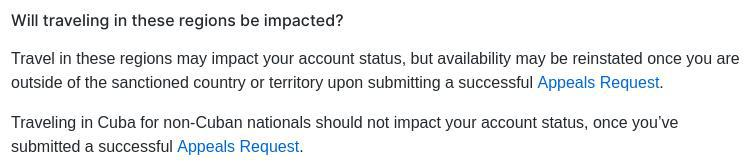
\includegraphics[width=.9\linewidth]{gorseller/github-amerika-yaptirimlari-2.jpg}
\caption{Üstelik bu ülkelere gitmiş ve oradan GitHub'a bağlanmışsanız, bu kısıtlamalar sizin hesabınıza da gelebilir ve tekrar hesabınızı açtırmak için o ülkelerden birinde yaşamadığınızı kanıtlamanız için \href{https://airtable.com/shrGBcceazKIoz6pY}{form doldurmanız} isteniyor. Formda istenen bilgilere baksanıza!}
\end{figure}

Levent Abi bir kez daha haklı çıktı, söylemi tekrar hatırlayalım: "Bulut
dediğin başkasının bilgisayarıdır. Bir gün gelir de, 'Sana hizmet vermiyorum
kardeşim' derse, öylece kalırsın ortada". Bir kere daha bulut sistemlere
güvenmememiz gerektiğini -umarım- öğrenmiş olduk. Güya internette gerçek
hayattaki gibi ülke sınırları yoktu, güya internetteyken fiziksel olarak
nerede olduğumuzun bir önemi yoktu\ldots{}
\section{PHP 7.4.0 \href{https://www.php.net/archive/2019.php\#2019-07-25-1}{Beta 1 yayınlandı}}
\label{sec:org6fca5c6}
22 Temmuz'da yeni özellik eklenmesi dondurulan (feature freeze) PHP 7.4'ün Beta
1 etiketine sahip ilk sürümü ise 25 Temmuz'da duyuruldu. PHP Wiki sayfasındaki
\href{https://wiki.php.net/todo/php74}{takvime göre} PHP 7.4.0 sürümün yayın sürecinin bu şekilde olması bekleniyor:

\begin{center}
\begin{tabular}{ll}
Tarih & Sürüm\\
\hline
08 Ağustos 2019 & Beta 2\\
22 Ağustos 2019 & Beta 3\\
05 Eylül 2019 & RC 1\\
19 Eylül 2019 & RC 2\\
03 Ekim 2019 & RC 3\\
17 Ekim 2019 & RC 4\\
31 Ekim 2019 & RC 5\\
14 Kasım 2019 & RC 6\\
28 Kasım 2019 & Final\\
\end{tabular}
\end{center}

PHP 7.4.0 ile gelecek bazı özellikler bu şekilde:
\subsection{Tipli sınıf özellikleri (\href{https://wiki.php.net/rfc/typed\_properties\_v2}{Typed Properties})}
\label{sec:org0d07af7}
PHP'de sınıf kodlarken artık sınıfın özelliklerini bu şekilde tipli
tanımlayabileceğiz:

\begin{minted}[breaklines=true,breakanywhere=true,frame=lines, linenos, label=PHP, labelposition=topline, startinline=true]{php}
class Kullanici {
    public int $id;
    public string $isim;

    public function __construct(int $id, string $isim) {
        $this->id = $id;
        $this->isim = $isim;
    }
}
\end{minted}
\subsection{\href{https://wiki.php.net/rfc/arrow\_functions\_v2}{Arrow Functions}}
\label{sec:org6789617}
Önceden bu şekilde olan kullanımı:

\begin{minted}[breaklines=true,breakanywhere=true,frame=lines, linenos, label=PHP, labelposition=topline, startinline=true]{php}
$sayilar = [1, 2, 3, 4, 5, 6];
$kareleri = array_map(function($sayi) { return $sayi * $sayi; }, $sayilar);
// 1, 4, 9, 16, 25, 36
\end{minted}

Artık bu formatta kullanabileceğiz:
\begin{minted}[breaklines=true,breakanywhere=true,frame=lines, linenos, label=PHP, labelposition=topline, startinline=true]{php}
$sayilar = [1, 2, 3, 4, 5, 6];
$kareleri = array_map(fn($sayi) => $sayi * $sayi, $sayilar);
// 1, 4, 9, 16, 25, 36
\end{minted}
\subsection{\href{https://wiki.php.net/rfc/null\_coalesce\_equal\_operator}{Null Coalescing Assignment Operator}}
\label{sec:org2a8d0b4}
Çevirisini yapamadım fakat bu operatör Türkiye'den birisi tarafından eklenen
bir özellik. Kendisini GitHub'da \href{https://github.com/midorikocak}{midorikocak} kullanıcı adıyla
bulabilirsiniz. Gelelim yeni operatörümüze, bu operatör sayesinde önceden bu
şekilde yazdığımız kod parçasını:

\begin{minted}[breaklines=true,breakanywhere=true,frame=lines, linenos, label=PHP, labelposition=topline, startinline=true]{php}
if (!isset($dizi['anahtar'])) {
    $dizi['anahtar'] = varsayilaniHesapla();
}
\end{minted}

Artık aşağıdaki gibi tek satırda yazabileceğiz:
\begin{minted}[breaklines=true,breakanywhere=true,frame=lines, linenos, label=PHP, labelposition=topline, startinline=true]{php}
$dizi['anahtar'] ??= varsayilaniHesapla();
\end{minted}

Bu katkısı için kendisine teşekkür ediyoruz.

Yazının fazla uzamaması için bu konuyu burada bırakıyorum ama eğer
ilgiliyseniz yeni özelliklerin tamamına \href{https://github.com/php/php-src/blob/php-7.4.0beta1/UPGRADING}{buradan erişebilirsiniz}.
\section{JDK 13 ile gelecek özellikler \href{https://www.javaworld.com/article/3341388/jdk-13-the-new-features-coming-to-java-13.html}{belli oldu}}
\label{sec:orgda286ab}
\href{../02/yazilim-gundemi-02.pdf}{Geçen haftaki gündemde} JDK 13 sürümünün "Rampdown" ikinci aşamaya geçtiğini
duyurmuştum. Bu hafta da yeni eklenecek bir özelliğe bakalım. Diğer özelliklere
de baktım fakat uzun zamandır Java yazmadığım için tam anlayamadım. Ben de
anladığım özelliği yazayım dedim :) Diğer özellik ve değişiklikler için konu
başlığına eklediğim bağlantıya tıklayabilirsiniz ya da QCon isimli konferansta
Oracle çalışanı Java Dil Mimarı Brian Goetz tarafından yapılan bu sunumu
izleyebilirsiniz: \href{https://www.infoq.com/presentations/java-futures-2019/}{Java Futures, 2019 Edition}.

\subsection{Çok satırlı String ifadeler}
\label{sec:org5a73d0d}
Önceden Java'da bir string değişken içerisine uzun bir ifade yazacağımız
zaman, bu şekilde bir yöntem izliyorduk:

\begin{minted}[breaklines=true,breakanywhere=true,frame=lines, linenos, label=Java, labelposition=topline]{java}
String html = "<html>" +
    "<body>" +
    "deneme" +
    "</body>" +
    "</html>";
\end{minted}
Bu şekilde bir kullanımda string parçaları birleştirildiği için biraz da olsa
performansı etkiliyordu fakat artık Python'da görmeye alıştığımız 3 tırnak
işaretli şu yapı Java'ya da geldi:

\begin{minted}[breaklines=true,breakanywhere=true,frame=lines, linenos, label=Java, labelposition=topline]{java}
String html = """
              <html>
                <body>
                  deneme
                </body>
              </html>
              """;
\end{minted}
\section{Apache NetBeans 11.1 \href{https://netbeans.apache.org/download/nb111/index.html}{duyuruldu}}
\label{sec:org20a40f4}
\begin{itemize}
\item Java EE 8 desteği,
\item \href{https://www.payara.fish/}{Payara} entegrasyonu,
\item GlassFish 5.0.1 desteği,
\item Tek dosya kaynak kodu programlarını çalıştırma (\href{https://openjdk.java.net/jeps/330}{PEP330: Launch Single-File
Source-Code Programs})
\item Fonksiyonun parametre isimlerini \href{https://github.com/apache/netbeans/pull/1247}{ipucu olarak gösterme}.
\item \texttt{switch} içerisindeki çoklu \texttt{case} kullanımı için \href{https://github.com/apache/netbeans/pull/1175}{kod tamamlama özelliği}
\end{itemize}

Eklenen diğer özelliklerin tam listesi ve detaylar için konu başlığındaki
bağlantıya tıklayabilirsiniz.
\section{Intellij IDEA 2019.2 \href{https://www.jetbrains.com/idea/whatsnew/\#v2019-2}{yayınlandı}}
\label{sec:orgbe52eaf}
\url{gorseller/intellij-idea-java-tekrarlayan-kod-dedektoru.gif}

NetBeans'e güncelleme gelir de, Intellij IDEA hiç geri kalır mı ?! Yapıştırmış
güncellemeyi:
\begin{itemize}
\item Java 13 desteği,
\item Otomatik tamamlama penceresi yanlış yazmalara karşı iyileştirilmiş,
\item Çalışan Docker konteynerindeki dosya sistemine erişme,
\item Açılış sürelerini kısaltan performans iyileştirmeleri,
\item Her klasörün kendine özel kod stili olabilecek,
\item 20'nin üzerinde dil için söz dizimi (syntax) renklendirme,
\end{itemize}

Eklenen diğer özelliklerin tam listesi ve detaylar için konu başlığındaki
bağlantıya tıklayabilirsiniz.
\section{Visual Studio 2019 \href{https://devblogs.microsoft.com/visualstudio/visual-studio-2019-version-16-2-generally-available-and-16-3-preview-1/}{16.2 ve 16.3 Preview 1 duyuruldu}}
\label{sec:orgcef2e30}
\begin{itemize}
\item Test Expolorer aracında iyileştirmeler,
\item Microsoft Edge Insider ile JavaScript hata ayıklama desteği,
\item C++ tarafında MSBuild projeleri için \href{https://devblogs.microsoft.com/cppblog/clang-llvm-support-for-msbuild-projects/}{Clang/LLVM desteği},
\item Daha fazla ekran alanını için tüm araç çubuklarını gizleyebilme
\end{itemize}

\begin{figure}[htbp]
\centering
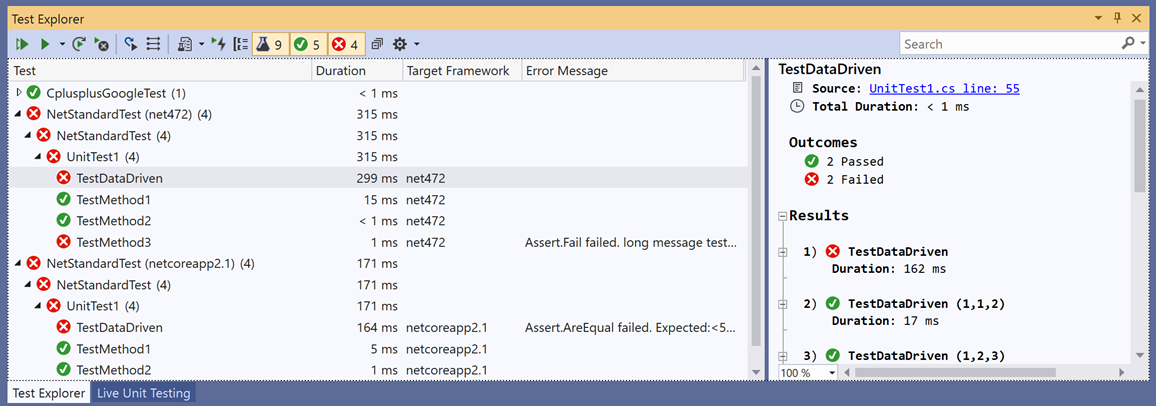
\includegraphics[width=.9\linewidth]{gorseller/visualstudio-yeni-test-explorer.png}
\caption{Yenilenmiş Test Explorer}
\end{figure}

Eklenen diğer özelliklerin tam listesi ve detaylar için konu başlığındaki
bağlantıya tıklayabilirsiniz.
\section{.NET Ekosistemi için güvenlik raporu \href{https://snyk.io/blog/net-open-source-security-insights/}{yayınlandı}}
\label{sec:orgc4bf8cf}
\begin{center}
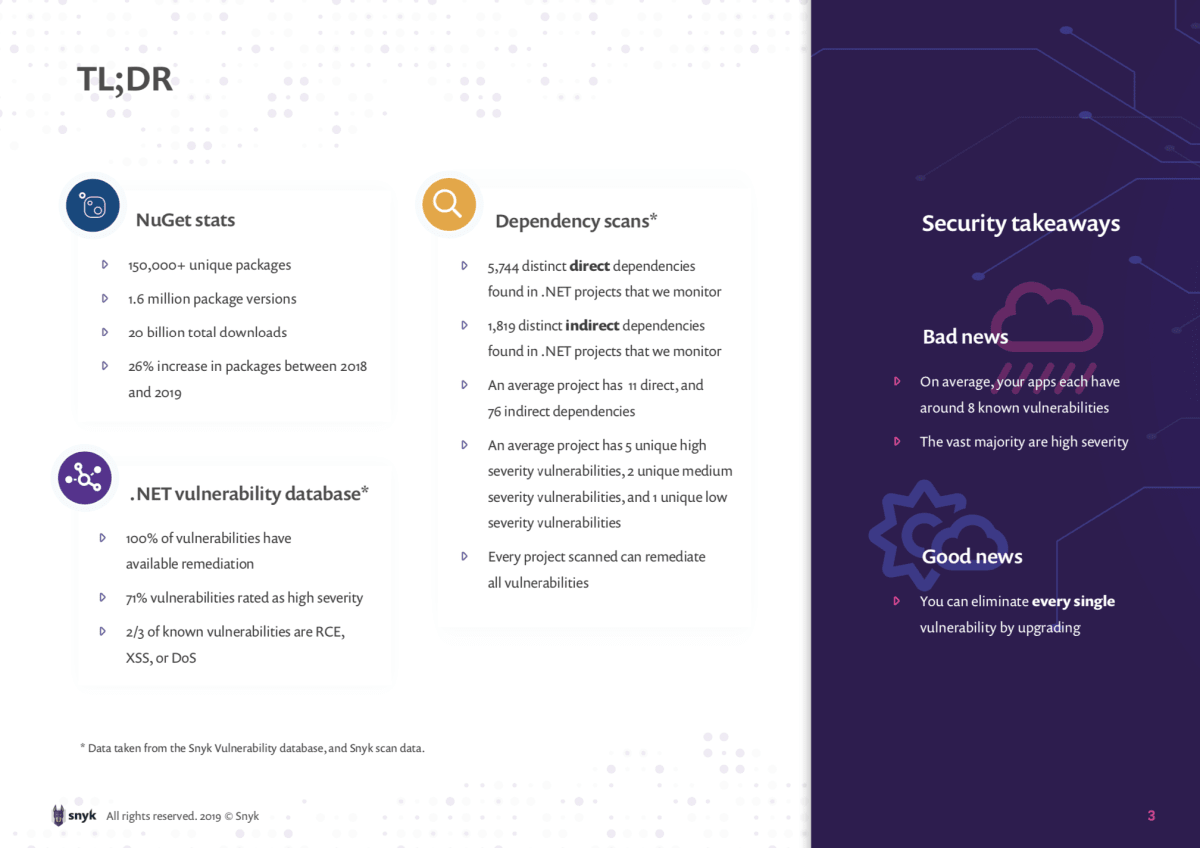
\includegraphics[width=.9\linewidth]{gorseller/dotnet-guvenlik-raporu-tldr.png}
\end{center}
\section{Diğer Haberler}
\label{sec:orgcf70396}
\begin{itemize}
\item FTP sunucusu ProFTPD'de güvenlik açığı tespit edildi: \href{https://tbspace.de/cve201912815proftpd.html}{CVE-2019-12815}.
\href{https://nvd.nist.gov/vuln/detail/CVE-2019-12815}{Alternatif}
\item Lyft, otonom araçlarının ham sensör verilerini \href{https://creativecommons.org/licenses/by-nc-sa/4.0/}{CC-BY-NC-SA-4.0} lisansı
altında paylaştı: \href{https://level5.lyft.com/dataset/}{Lyft Level 5 AV dataset}.
\item GitLab 12.1 sürümü \href{https://about.gitlab.com/2019/07/22/gitlab-12-1-released/}{yayınlandı}
\item .NET Core 3.0 Preview 7 \href{https://devblogs.microsoft.com/dotnet/announcing-net-core-3-0-preview-7}{duyuruldu}.
\item Microsoft, metin analiz ve görselleştirme aracını açık kaynak olarak
yayınlandı: \href{https://github.com/microsoft/browsecloud}{browsecloud}
\item Microsoft, OpenAI organizasyonuna 1 milyar dolar \href{https://openai.com/blog/microsoft/}{yatırım yaptı}.
\item Microsoft Security Response Centre, Rust ile ilgili ilk blog yazısını
yayınladı: \href{https://msrc-blog.microsoft.com/2019/07/22/why-rust-for-safe-systems-programming/}{Why Rust for safe systems programming}
\item SQL Server 2019 CTP 3.2 sürümü \href{https://cloudblogs.microsoft.com/sqlserver/2019/07/24/sql-server-2019-community-technology-preview-3-2-is-now-available/}{duyuruldu}.
\item Julia programlama dili \href{https://julialang.org/blog/2019/07/multithreading}{'composable multi-thread parallelism' özelliği} kazandı.
\item Rust derleyicisi \href{https://blog.mozilla.org/nnethercote/2019/07/25/the-rust-compiler-is-still-getting-faster/}{hızlanmaya devam ediyormuş}.
\item Paralel programlama sistemi \href{https://legion.stanford.edu/overview/}{Legion}, \href{https://github.com/StanfordLegion/legion/releases/tag/legion-19.06.0}{19.06.0 sürümünü duyurdu}.
\item Geliştiricisi \href{https://inductive.no/jai/}{Jai programlama dili} için \href{https://www.youtube.com/watch?v=4\_ODvZ01CjU}{durum raporu videosu} hazırlamış. Bu
programlama dili Twitch platformunda canlı yayınlarda geliştiriliyor.
Geliştiricinin twitch kanalı: \url{https://www.twitch.tv/naysayer88}
\item Amazon'un sesden yazı elde etme hizmeti Amazon Transcribe, artık \href{https://aws.amazon.com/blogs/aws/amazon-transcribe-streaming-now-supports-websockets/}{WebSockets
destekliyor}.
\item Mozilla IoT takımı, WebThings projesi altında geliştirdikleri WebThings
Gateways aracının 0.9 sürümünü \href{https://venturebeat.com/2019/07/25/mozilla-debuts-webthings-gateway-open-source-router-firmware-for-turris-omnia/}{duyurdu}. \href{https://github.com/mozilla-iot/gateway}{GitHub Deposu}
\item Google Chrome tarayıcısının \href{https://medium.com/kulak/changes-in-web-midi-api-in-chrome-in-2019-4e410ec76af}{Web MIDI API sisteminde değişiklik var}.
\item OpenJDK takımı, Project Valhalla LW2 Prototipini \href{https://www.infoq.com/news/2019/07/valhalla-openjdk-lw2-released/}{duyurdu}.
\item Git istemcisi Fork \href{https://fork.dev/releasenotes}{1.0.82 sürümünü duyurdu}.
\item Python için video işleme kütüphanesi olan VidGear, \href{https://github.com/abhiTronix/vidgear/releases/tag/vidgear-0.1.5}{v0.1.5 sürümünü duyurdu}.
\item Go yorumlayıcı projesi açık kaynak olarak yayınlandı: \href{https://blog.containo.us/announcing-yaegi-263a1e2d070a}{yaegi}. \href{https://github.com/containous/yaegi}{GitHub Deposu}
\item Tek Sayfalık Uygulamalar (Single Page Applications) için geliştirilmiş
framework mithil.js \href{https://github.com/MithrilJS/mithril.js/releases/tag/v2.0.1}{v2.0.1 sürümünü yayınladı}.
\item Bellek üzerinde hassas verileri depolamaya yarayan Go kütüphanesi MemGuard,
v0.18.1 sürümünü \href{https://github.com/awnumar/memguard/releases/tag/v0.18.1}{duyurdu}.
\item Rust ile platformlar-arası grafiksel kullanıcı arayüzleri geliştirmeye
olanak sağlayan kütüphane açık kaynak olarak yayınlandı: \href{https://github.com/ivanceras/sauron-native}{Sauron-native}
\item C/C++ için platformlar arası (cross-platform) paket yöneticisi Hunter,
v0.23.205 \href{https://github.com/ruslo/hunter/releases/tag/v0.23.205}{sürümünü duyurdu}.
\item Tüm projeler ve sistemler için evrensel proje yöneticisi olma iddiası
taşıyan GuPM isimli araç 1.2.0 \href{https://github.com/azukaar/GuPM/releases/tag/1.2.0}{sürümünü duyurdu}.
\item Sinuous UI kütüphanesinin v0.12.5 \href{https://github.com/luwes/sinuous/releases/tag/v0.12.5}{sürümü çıktı}.
\item SQL raporlama aracı Poli v0.9.0 \href{https://github.com/shzlw/poli/releases/tag/v0.9.0}{sürümü yayınlandı}.
\end{itemize}
\section{Lisans}
\label{sec:org7c59a0f}
\begin{center}
\begin{center}

\includegraphics[height=1.5cm]{../../../img/CC_BY-NC-SA_4.0.png}
\end{center}

\href{yazilim-gundemi-03.pdf}{Yazılım Gündemi - 3} yazısı \href{https://erenhatirnaz.github.io}{Eren Hatırnaz} tarafından \href{http://creativecommons.org/licenses/by-nc-sa/4.0/}{Creative Commons
Atıf-GayriTicari-AynıLisanslaPaylaş 4.0 Uluslararası Lisansı} (CC BY-NC-SA 4.0)
ile lisanslanmıştır.
\end{center}
\end{document}
